\section{Part C}

\begin{enumerate}[label=Question \arabic*.]
\item I ensure the resource are efficiently used by monitoring the Spark dashboard. As shown in \figurename~\ref{fig:res_use}, all cores of the four workers are active and each worker has 1GB memory in use.

\begin{figure}
    \centering
    \includegraphics[width=7in]{PartC/resource_utilization.png}
    \caption{Caption}
    \label{fig:res_use}
\end{figure}

Regarding the network bandwidth, I only compute the transmit size as the transmit time cannot be estimated from the application completion time. More precisely, computing the bandwidth is in fact computing the throughput (TransmitSize / IOTime). Assume the latency is negligible, the bandwidth is approximately equal to the throughput. Each configuration are run three times and the average value is taken. I vary the partitioning size (\tablename{~\ref{tab:q4:RDD2}-~\ref{tab:q4:RDD300}}). From the results, 10 partitions in RDD has the minimum completion time. I will choose RDD partitioning size = 10 for question 2 and question 3. 

    \begin{table}[!h]
        \centering
        \begin{tabular}{|c|c|c|c|c|c|c|c|}
        \hline
            \multirow{2}{*}{hosts} & \multirow{2}{*}{Completion time (s)} & \multicolumn{2}{|c|}{Network Transmit Size (MiB)} & \multicolumn{2}{|c|}{Disk Bandwidth (MB/s)} & \multirow{2}{*}{Number of tasks} \\ 
            \cline{3-6}
    & & Receive & Transmit & Read & Write &  \\
        \hline
            vm-21-1 & \multirow{5}{*}{75.0}  & 1.47 & 1.12 & 4.15 & 1.40 & \multirow{5}{*}{23}  \\
            vm-21-2 &  & 0.32 & 112.52 & 9.36 & 1.63 &  \\
            vm-21-3 &  & 0.09 & 0.24 & 4.58 & 1.74 &  \\
            vm-21-4 &  & 117.25 & 0.78 & 4.10 & 4.23 &  \\
            vm-21-5 &  & 0.09 & 0.24 & 4.70 & 1.16 &  \\
        \hline
        \end{tabular}
        \caption{Qeustion 1 Page Rank}
        \label{tab:q1}
    \end{table}
    
    
    \item I use two customed partitions, RangePartitioner and HashPartitioner. The metrics are shown in \tablename{~\ref{tab:q2:hash},~\ref{tab:q2:range}}. The application completion times with and without customed partitioning are nearly the same. Regarding the page rank algorithm, the customed partitioning is slightly faster. However there is an overhead to partition the data. For Range partitioner, the application consists of two jobs. One is range partitioning, which takes 16s. The other is pagerank, which takes 29s.
    
    \begin{table}[!h]
    	\centering
    	\begin{tabular}{|c|c|c|c|c|c|c|c|}
    		\hline
    		\multirow{2}{*}{hosts} & \multirow{2}{*}{Completion time (s)} & \multicolumn{2}{|c|}{Network Transmit Size (MiB)} & \multicolumn{2}{|c|}{Disk Bandwidth (MB/s)} & \multirow{2}{*}{Number of tasks} \\ 
    		\cline{3-6}
    		& & Receive & Transmit & Read & Write &  \\
    		\hline
    		vm-21-1 & \multirow{5}{*}{41.9}  & 3.70   & 3.25   & 4.14 & 1.49 & \multirow{5}{*}{225}  \\
    		vm-21-2 &                        & 140.83 & 255.12 & 7.08 & 2.37 &  \\
    		vm-21-3 &                        & 208.00 & 64.79  & 3.36 & 3.12 &  \\
    		vm-21-4 &                        & 144.78 & 291.07 & 3.66 & 2.51 &  \\
    		vm-21-5 &                        & 199.62 & 58.62  & 3.41 & 3.43 &  \\
    		\hline
    	\end{tabular}
    	\caption{Qeustion 2 Page Rank with Hash Partitioner}
    	\label{tab:q2:hash}
    \end{table}
    
    \begin{table}[!h]
       	\centering
       	\begin{tabular}{|c|c|c|c|c|c|c|c|}
       		\hline
       		\multirow{2}{*}{hosts} & \multirow{2}{*}{Completion time (s)} & \multicolumn{2}{|c|}{Network Transmit Size (MiB)} & \multicolumn{2}{|c|}{Disk Bandwidth (MB/s)} & \multirow{2}{*}{Number of tasks} \\ 
       		\cline{3-6}
       		& & Receive & Transmit & Read & Write &  \\
       		\hline
    		vm-21-1 & \multirow{5}{*}{45.2}  & 3.00   & 3.02   & 4.28 & 1.31 & \multirow{5}{*}{227}  \\
    		vm-21-2 &                        & 121.97 & 228.55 & 8.26 & 2.52 &  \\
    		vm-21-3 &                        & 176.77 & 55.26  & 3.52 & 2.91 &  \\
    		vm-21-4 &                        & 143.68 & 250.42 & 3.81 & 2.53 &  \\
    		vm-21-5 &                        & 168.06 & 55.06  & 3.67 & 3.21 &  \\
       		\hline
       	\end{tabular}
       	\caption{Qeustion 2 Page Rank with Range Partitioner}
       	\label{tab:q2:range}
    \end{table}

    
    \item As there is no improvement using the customed partitioning, in this question I use the partitioning scheme in Question 1. Fix the RDD partition size as 10, cache the variable graph. The experimental result is in \tablename~\ref{tab:q3}. The application with cached graph is only 0.4s faster than the uncached one. The reason is not clear. I suspect Spark do some optimization by automatically storing the graph variable in memory.
    \begin{table}[!h]
        \centering
        \begin{tabular}{|c|c|c|c|c|c|c|c|}
        \hline
            \multirow{2}{*}{hosts} & \multirow{2}{*}{Completion time (s)} & \multicolumn{2}{|c|}{Network Transmit Size (MiB)} & \multicolumn{2}{|c|}{Disk Bandwidth (MB/s)} & \multirow{2}{*}{Number of tasks} \\ 
            \cline{3-6}
    & & Receive & Transmit & Read & Write &  \\
        \hline
            vm-21-1 & \multirow{5}{*}{41.8}  & 3.06   & 2.98   & 4.36 & 1.35 & \multirow{5}{*}{215}  \\
            vm-21-2 &                        & 188.82 & 158.37 & 8.70 & 3.01 &  \\
            vm-21-3 &                        & 185.58 & 45.10  & 4.66 & 2.67 &  \\
            vm-21-4 &                        & 121.92 & 406.97 & 4.09 & 2.17 &  \\
            vm-21-5 &                        & 181.96 & 44.66  & 4.82 & 2.72 &  \\
        \hline
        \end{tabular}
        \caption{Qeustion 3 Page Rank}
        \label{tab:q3}
    \end{table}
    
    \item In this question, I experimented over four different paritionings i.e. 2, 10, 100, 300. From the results (\tablename~\ref{tab:q4:RDD2}-\ref{tab:q4:RDD300}), when RDD partition size is 10 the applicaton completion time is minimum. When the partition size increases, the parallelism increases so that the application completion time decrease. However, when the partition size are too large, the network transmit overhead will dominate and make the application completion time longer.
    
         \begin{table}[!h]
        \centering
        \begin{tabular}{|c|c|c|c|c|c|c|c|}
        \hline
            \multirow{2}{*}{hosts} & \multirow{2}{*}{Completion time (s)} & \multicolumn{2}{|c|}{Network Transmit Size (MiB)} & \multicolumn{2}{|c|}{Disk Bandwidth (MB/s)} & \multirow{2}{*}{Number of tasks} \\ 
            \cline{3-6}
        & & Receive & Transmit & Read & Write &  \\
        \hline
            vm-21-1 & \multirow{5}{*}{81.6}  & 1.43   & 1.35   & 4.60 & 1.66 & \multirow{5}{*}{47}  \\
            vm-21-2 &                        & 94.57  & 191.65 & 9.37 & 2.48 &  \\
            vm-21-3 &                        & 94.26  & 79.12  & 4.50 & 2.57 &  \\
            vm-21-4 &                        & 362.50 & 271.52 & 4.01 & 2.96 &  \\
            vm-21-5 &                        & 94.05  & 78.73  & 4.93 & 2.35 &  \\
        \hline
        \end{tabular}
        \caption{Qeustion 4 Number pf partitions = 2}
        \label{tab:q4:RDD2}
        
        \begin{tabular}{|c|c|c|c|c|c|c|c|}
        \hline
            \multirow{2}{*}{hosts} & \multirow{2}{*}{Completion time (s)} & \multicolumn{2}{|c|}{Network Transmit Size (MiB)} & \multicolumn{2}{|c|}{Disk Bandwidth (MB/s)} & \multirow{2}{*}{Number of tasks} \\ 
            \cline{3-6}
        & & Receive & Transmit & Read & Write &  \\
        \hline
            vm-21-1 & \multirow{5}{*}{42.2}  & 3.07   & 2.88   & 5.00 & 1.79 & \multirow{5}{*}{215}  \\
            vm-21-2 &                        & 222.59 & 175.95 & 9.04 & 2.94 &  \\
            vm-21-3 &                        & 174.27 & 71.74  & 4.77 & 2.83 &  \\
            vm-21-4 &                        & 180.48 & 398.66 & 3.97 & 2.30 &  \\
            vm-21-5 &                        & 166.13 & 70.75  & 4.68 & 3.32 &  \\
        \hline
        \end{tabular}
        \caption{Qeustion 4 Number pf partitions = 10}
        \label{tab:q4:RDD10}
        
        \begin{tabular}{|c|c|c|c|c|c|c|c|}
        \hline
            \multirow{2}{*}{hosts} & \multirow{2}{*}{Completion time (s)} & \multicolumn{2}{|c|}{Network Transmit Size (MiB)} & \multicolumn{2}{|c|}{Disk Bandwidth (MB/s)} & \multirow{2}{*}{Number of tasks} \\ 
            \cline{3-6}
        & & Receive & Transmit & Read & Write &  \\
        \hline
            vm-21-1 & \multirow{5}{*}{50.8}  & 18.24  & 18.96  & 5.53 & 3.31 & \multirow{5}{*}{2105}  \\
            vm-21-2 &                        & 235.60 & 275.60 & 8.94 & 2.29 &  \\
            vm-21-3 &                        & 190.84 & 139.12 & 4.80 & 2.60 &  \\
            vm-21-4 &                        & 407.09 & 504.37 & 3.74 & 2.46 &  \\
            vm-21-5 &                        & 274.00 & 154.27 & 4.79 & 2.84 &  \\
        \hline
        \end{tabular}
        \caption{Qeustion 4 Number pf partitions = 100}
        \label{tab:q4:RDD100}
        
        \begin{tabular}{|c|c|c|c|c|c|c|c|}
        \hline
            \multirow{2}{*}{hosts} & \multirow{2}{*}{Completion time (s)} & \multicolumn{2}{|c|}{Network Transmit Size (MiB)} & \multicolumn{2}{|c|}{Disk Bandwidth (MB/s)} & \multirow{2}{*}{Number of tasks} \\ 
            \cline{3-6}
        & & Receive & Transmit & Read & Write &  \\
        \hline
            vm-21-1 & \multirow{5}{*}{80.8}  & 54.41  & 56.77  & 4.21 & 4.69 & \multirow{5}{*}{6305}  \\
            vm-21-2 &                        & 461.86 & 443.06 & 8.77 & 1.89 &  \\
            vm-21-3 &                        & 456.85 & 316.62 & 4.38 & 1.93 &  \\
            vm-21-4 &                        & 467.47 & 728.71 & 3.94 & 2.28 &  \\
            vm-21-5 &                        & 456.67 & 328.13 & 4.45 & 2.05 &  \\
        \hline
        \end{tabular}
        \caption{Qeustion 4 Number pf partitions = 300}
        \label{tab:q4:RDD300}
    \end{table}
    
    
    \item See \figurename~\ref{fig:q5}. Same for all three application because they have the same algorithm. The difference in the partitioning and cache does not have an impact on the lineage graph.
    
    \begin{figure}
	     \centering
	     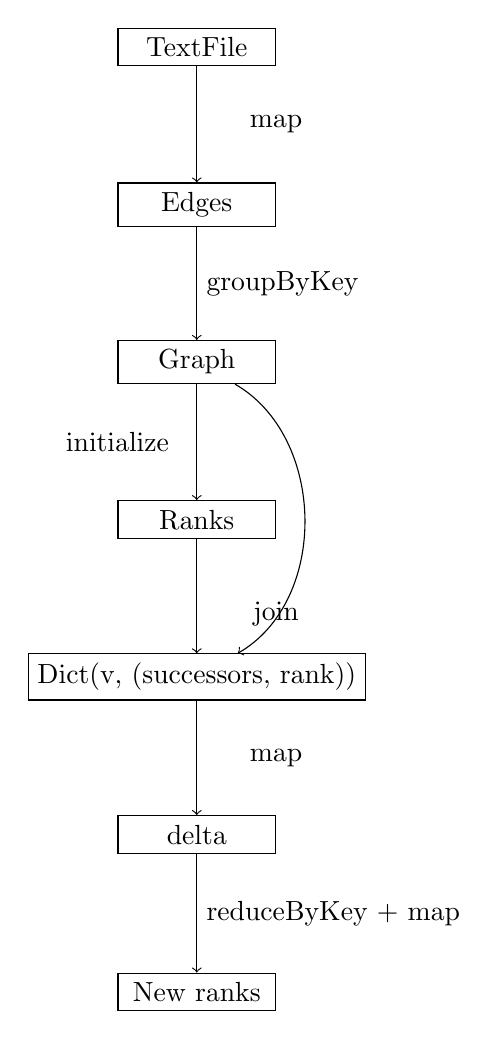
\begin{tikzpicture}[node distance=2cm, minimum width=2cm]
		     \node[draw, rectangle] (tx) {TextFile};
		     \node[draw, rectangle, below of=tx] (ed) {Edges};
		     \node[draw, rectangle, below of=ed] (g) {Graph};
		     \node[draw, rectangle, below of=g] (r) {Ranks};
		     \node[draw, rectangle, below of=r] (d) {Dict(v, (successors, rank))};
		     \node[draw, rectangle, below of=d] (delta) {delta};
		     \node[draw, rectangle, below of=delta] (newRank) {New ranks};
		     
		     \draw[->] (tx) -- (ed) node[midway, right] {map};
		     \draw[->] (ed) -- (g) node[midway, right] {groupByKey};
		     \draw[->] (g) -- (r) node[midway, left] {initialize};
		     \draw[->] (r) -- (d) node[pos=0.66, right] {join};
		     \draw[->] (g) to[out=-30,in=30] (d);
		     \draw[->] (d) -- (delta) node[midway, right] {map};
		     \draw[->] (delta) -- (newRank) node[midway, right] {reduceByKey + map};
	     \end{tikzpicture}
        \caption{Lineage graph for Question 3}
        \label{fig:q5}
    \end{figure}
    
    \item \figurename~\ref{fig:q6}. All applications have the same DAGs. The reason is they share the same repartitioning size (10) and the same algorithm. Impact: if we have a repartition step, we will distributed the data across the workers so all the workers will be used. This increases parallelism and speeds up the application.
    
    \begin{figure}
        \centering
        \begin{minipage}[t]{0.19\textwidth}
        \includegraphics[width=1in]{PartC/DAGs/CQ2S0.png}
        \subcaption{Stage 0}
        \end{minipage}
        \begin{minipage}[t]{0.19\textwidth}
        \includegraphics[width=1in]{PartC/DAGs/CQ2S1.png}
        \subcaption{Stage 1}
        \end{minipage}
        \begin{minipage}[t]{0.19\textwidth}
        \includegraphics[width=1in]{PartC/DAGs/CQ2S2.png}
        \subcaption{Stage 2}
        \end{minipage}
        \begin{minipage}[t]{0.19\textwidth}
        \includegraphics[width=1in]{PartC/DAGs/CQ2S4.png}
        \subcaption{Stage 4}
        \end{minipage}
        \begin{minipage}[t]{0.19\textwidth}
        \includegraphics[width=1in]{PartC/DAGs/CQ2S6.png}
        \subcaption{Stage 6}
        \end{minipage}
        \caption{Question 2/3 Stage-level DAGs}
        \label{fig:q6}
    \end{figure}
   
    
\item In this question, I failed vm-21-4 for all cases. The result is in \tablename~\ref{tab:q7}. The impact of clearing cache is not obvious. The spark jobs are executed as the normal case. However killing one running worker increase the completion time much, especially when the failure is at 75\% progress. The reason is on killing the worker, the ongoing stage failed and Spark will retry it on other workers. For example, in the case where the failure b happens at 75\% for question 1's app,  to deal with the failure, spark runs 7 more stages (14 more tasks) and the overhead is about 35s.
    
    \begin{table}[!t]
        \centering
        \begin{tabular}{c|c|c|c|c}
        \hline
            & failure a at 25\% & failure a at 75\% & failure b at 25\% & failure b at 75\% \\
        \hline
           Q1 & 71.3s & 75.3s & 73.3s & 108.4s \\
       Q3 & 44.2s & 42.2s & 52.2s & 54.2s \\
        \hline
        \end{tabular}
        \caption{Completion time}
        \label{tab:q7}
    \end{table}
    
    
\end{enumerate}